\chapter{Preliminaries}
\label{Preliminaries}
%\section{Graph Notations}
%\begin{mydef}
%A graph $G$ ist defined by a tuple $(V,E)$ with $V$ being a set of Verticies and $E$ a set of Edges.
%$V = (v_{1}, ..., v_{n})$
%\begin{enumerate}
% \item A graph is directed if the elements in $E$ consists out of tuples.\\
% $E = \{(v_{i},v_{j}),..\}$ for $v_{i},v_{j} \in V$ with $v_{i} \neq v_{j}$
% \item A graph is undirected if the elements in $E$ consists out of sets with the size of 2.\\
% $E = \{\{v_{i},v_{j}\},..\}$ for $v_{i},v_{j} \in V$ with $v_{i} \neq v_{j}$
%\end{enumerate}
%\end{mydef}
%This definition is based on \cite{Diestel.2012}. If $\{v_{i},v_{j}\} \in E$ then $v_{i}$ and $v_{j}$ are neighbors. In a directed graph the direction of the edge matters, if $(v_{i},v_{j}) \in E$ %then $v_{i}$ is a neigbor of $v_{j}$, but not the other way around.
%\begin{mydef}
%A graph $G$ is called a
%\begin{enumerate}
% \item Multigraph if it contains multiple edges between the same vertices or edges from a vertex to the same vertex.
% \item Hypergraph if it contains edges, which have more than two vertices connected to it.
%\end{enumerate}
%\end{mydef}
%\newpage
\section{Graph File Formats}
A graph file format is a specification for describing a graph in a predefined syntax, which then can be read in by an application to access the data. Over the course of time many graph file formats have been established. Most of these formats were developed, with a special use cases in mind. For example GraphML was designed to support as many features as possible for graph drawing\cite{Roughan.10.03.2015}.
In the recent time the trend to invent new graph formats is decreasing. It can be seen in \cite{Roughan.10.03.2015} that most of the formats, which get listed in their work, aren't developed any further, also there is an significant reduction of xml type formats in the last couple of years and the number of json graph file formats is rising.
Based on the collection provided in \cite{Roughan.10.03.2015}, a table with formats was created to identify their up-to-dateness.

\begin{table}[H]
\begin{center}
    \begin{tabular}{| l | l | l | l |}
    \hline
	\bfseries Id & \bfseries Graph File Format & \bfseries Reference Time Frame & \bfseries Structure\\ \hline
	1 & GraphML & 2000 - present & XML\\ \hline
	2 & JSON Graph & 2014 - present & JSON\\ \hline
	3 & KrackPlot & 1993 - present & simple\\ \hline
	5 & Ordered Graph Data Language & 2002 - present & BNF\\ \hline
	6 & Open Graph Markup Language & 2012 - present & XML\\ \hline
	7 & Simple Interaction Format & 2003 - present & simple\\ \hline
	8 & Stanford Network Analysis Platform & 2005 - present & simple\\ \hline
	9 & Trival Graph Format & unknow - present & simple\\ \hline
    \end{tabular}
\end{center}\caption{Selection of up-to-date Graph File Formats based on\cite{Roughan.10.03.2015} and their specifications.\newline}
\label{tabelle_avarage_time}
\end{table}
 There are several properties, which an graph file format has to fulfill. For example, not all formats are a good option for big data sets. XML and even JSON formats have an bigger overhead then just a simple edge list \cite{JSONvsXML}. This overhead scales with the size of the data and can have an impact on the performance of the loading. Our file formats have to be scalable, otherwise just small datasets are supported and this results in probably faster loading times on a single peer. Most big data sets are provided in simple formats and resolve around saving space, but keeping the format as simple as possible.
 Also there file formats that don’t provide any clear specifications the development has been stopped. This is a problem for more complex formats, because this could lead to inconsistencies while loading or reading these format files. 
 For more simple formats, which follow a trivial approach, is often no specification needed, because their simplicity makes them self-explanatory.

\subsection{Division of Formats}
To enable distributed loading, the graph file format needs to be split into multiple chunks \cite{parallelGraphLoading}, which then can be distributed inside the distributed system. The goal is to gain performance, while parallel processing the data on multiple nodes. To be able to split the file, an section must be identified, so that the information inside this chunks doesn't lose it current context. A chunk without its context, can't be interpreted correctly and will unavoidable lead to an wrong graph. If the context isn't keep-able, then loading the format on an single node is probably the best workaround.\\
It isn't surprising that most formats are divisible in some way, but the main factor to consider at this point, is performance. All peers must wait for the chunks to be created, thats why is in this step no interpretation of the file should be done. This isn't avoidable for all formats, but for the most simple formats there is a way split files without or minimal reading of the file itself.\\
To determine if a format is divisibility the structure of the file needs to be specified and analyzed. Most important data inside the file shouldn't be dependent on other sections of the same file. In other words the chunks should contain all needed data for reading. 
There will be formats that specify information about vertices in multiple sections of the file, but this information needs to be independent. If the following data can only be processed after processing all lines before, then this section can't be split. Sections that can't be split for example are edge-tuples, this sections will be referred to as indivisible sections.\\
These indivisible sections are often surrounded or closed by separators. An separator could be anything often newline characters, tabulations and  semicolons are used, but also tags (XML), brackets (JSON) or even the position itself in binary sequences can be used to divide these sections. Some formats provide meta data, that will help split up files by defining the position of the information and their format.\\
A format is fully divisible if it could be split at the any separator, this will mostly be true for simple formats.

\subsection{Simple Formats}
Simple formats are often a trivial approach of creating an low level but highly function graph file format. These formats are often self-explanatory, but have no official specification. This leads to various problems, beacuse it isn’t clear where the boundaries of this formats are. For example which character set is used, which separator is used or if the format contains meta data/comments\cite{Roughan.10.03.2015}.\\
Many of these formats are fully divisible, duo to the fact that they often only contain small indivisible sections, so that these sections can be grouped and stored in chunks. Also leads their simplicity to an plain hierarchy inside the file.

\subsubsection{Trivial Graph Formats}
As trivial graph file formats(TGF) are referred to a list of formats, that follow an simple implementation, but have no specification. The most common formats are standard approaches like edge lists, adjacency matrices, neighbor lists and path list.\\

\noindent{\textit{Edge List}}\\
The Edge list is the most common and trivial approach , of storing a graph.
This format is just an list of all edges of the graph. In most cases one line equals one edge, so lines form an indivisible section. After each line the file could be split.
One line is made of two edges, which a separated by an separator. Often tabulations are used here, but also spaces and other characters could be used. This format has a relatively low overhead and scales well.\\

\noindent{\textit{Binary Edge List}}\\
This is an compressed version of the Edge List, where no lines are used instead all edges have an fixed size for example the first 8 bytes indicate the start vertex and the follow 8 bytes the target vertex. This compression leads to the advantage that no separator is used, so there is no overhead, but the human readability is lost.\\

\noindent{\textit{Adjacency Matrix}}\\
The adjacency matrix is an matrix, where each entry represents an edge connection between the according vertices. The vertices are identified via row and column number, but often these numbers are left out, to safe space and the rows and lines read in previously need to be counted. The biggest flaw of this format is that it doesn't scale well for big data sets, duo to the fact that every vertex got an entry for every other vertices. So its size increases squarely to the amount of vertices.\\

\noindent{\textit{Neighbor List}}\\
The Neighbor List is is a combination of an Adjacency Matrix and an Edge List, but it removes the unnecessary entires for each vertex. Each row describes all connections for a vertex, so we end up with one line per vertex. This format scales better then the Edge List, duo to the fact that vertices are identified through lines.\\

\noindent{\textit{SNAP Format}}\\
The SNAP format just makes an simple addition to the edge list, by allowing comments inside the file. These are identified through a hashtag at the beginning of the line.\\

\noindent{\textit{Edge/Vertex-List with Properties}}\\
This Format consists out of two files, one file contains just list of vertices. The other file contains an Weighted Edge List with an weight value for each edge at the end of the line. This format is used by the LDBC-Graphalytics Benchmark.\cite{LDBC-Graphalytics}

\begin{figure}[H]
	\centering
	[Graphic]\\
	%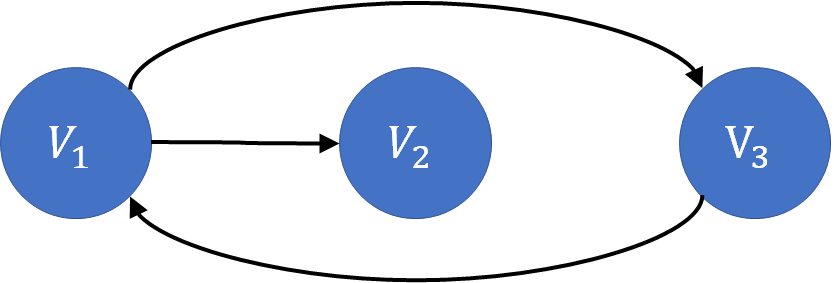
\includegraphics[height=4cm]{img/simple.png}
	\label{simple}
		\setlength{\tabcolsep}{0.5cm} % Abstand zwischen den Spalten einer Tabelle
		\begin{tabular}{lllll}
			\\
			adjacency matrices & neighbor list & edge list & path list \\
			$A = \left( \begin{array}{rrr}0 & 1 & 1 \\0 & 0 & 0 \\1 & 0 & 0\\\end{array}\right)$ &$\begin{array}{lll}1, 2\\1, 3\\3, 1\\\end{array}$ &$\begin{array}{lll}2,3 \\\\1\\\end{array}$ &$\begin{array}{lll}3,1,2 \\ 1,3 \\\end{array}$ \\
			
		\end{tabular}
	\caption{An example graph with three vertices in different trivial graph formats\cite{Roughan.10.03.2015}}
\end{figure}

		

\subsubsection{SIF Format}
The SIF Format is a combination of an edge list with a neighbor list. Additionally, the type of connection can be specified with strings. It allows multiple edges between the same nodes, if the connection type varies, otherwise it is specified to ignore duplicates. One downside is that the format allows tabulations or spaces as separators, it is stated that if no tabulations are used in the whole file spaces are used as separators, but because all lines have an equal format, it can be stated, if the first line doesn't contain any tab character, spaces will be used as separators. Based of the fact that SIF is combination of two TGFs, it can be said that SIF is also fully divisable, only one separator is used per file and the lines are indivisible sections between which can be split. \cite{TheCytoscapeConsortium.2017}

\subsubsection{KrackPlot 3.0}
KrackPlot 3.0 follows for simple formats a more complex syntax then the TGFs. The first line contains the number of nodes specified in the following data. This information helps with various problems, like splitting nodes appropriately into chunks. The next line can contain two options “!nc” or “!nl”. The first option specifies that the following data contains no coordinates, the other one declares that no labels will be specified. If labels and/or coordinates are defined they start on the second line until line (node-amount)+1. After the second line or the labels/coordinates an adjacency matrix specifies the connections of the nodes.
This format doesn't scale well for big data sets duo to its adjacency matrix, but splitting this format would be rather easy duo to the fact that the number of nodes is known and only two lines need to be read in, to know the whole nature of the file.\cite{D.KrackhardtJ.BlytheC.McGrath.4.12.2001}\\ 

\subsection{XML Formats}
There are various implementations of graph file formats using XML. The XML format is based around tags, which define the object it is describing. It is a structure descriptive language for hierarchically structured data. Reading its information is as result not line based rather it is tag based. This format is hard to divide without reading it completely, because the XML format consists of multiple layers. This results in the problem to determine the layer on which the object is located, this problem can only be solved by counting the opened and closed tags or using a flat hierarchy.\cite{bray1997extensible,Roughan.10.03.2015}
The XML language provides an much higher overhead as the simple graph file formats, which results in an increased file size and as a consequence increased loading time.

\subsubsection{GraphML}
GraphML is an XML based graph file format. It consists out of one graph element which can contain unordered node and edge elements. GraphML supports hyperedges and nested networks and much more graph features. This results in the problem of deep hierarchies, which can only be solved by tag counting do determine the layer. GraphML support many kinds of graphs, this variety causes many different cases to consider. GraphML doesn't specify the positions of vertices or edges inside the format, so that chunks could result in an unequal distribution of different objects. This results in extracting information while reading the file, which will result in a much more time consumption.\cite{brandes2013graph,kuhner2013graphml}

\subsubsection{Open Graph Markup Language}
The Open Graph Markup Language is part of the Open Graph Drawing Framework. The OPML got some similarities to GraphML, duo to the fact that both formats resolve around XML. Also, this format implements many graph style and drawing operations. Also the OPML doesn’t support nested graphs unlike GraphML, which results in a flatter hierarchy.\cite{opengraph.format}

\subsubsection{Resource Description Framework}
The Resource Description Framwork/XML Format isn't meant to be an graph format, but is commonly used for smaller graphs. Its defines objects and attributes via namespaces. The main feature of this format is its portability duo its model of three information types, which can be mapped as network.\cite{miller1998introduction,Lassila98resourcedescription}

\subsection{JSON Graph}
JSON Graph is based on the JSON-syntax-specification, which allows this fomrat to be read in by normal JSON parsers. This format defines first an graph object, which contains an array of mutiple other object. JSON Graph specifies that every graph object contains an array of nodes and an array of edges. Edges alaways contain the fields source node and target node. Nodes always contain a unique key, which identifies them. All field are JSON Strings.\\
To load this format it can be assumed, that our graphs do not contain any meta data. This leads to lower oberhead then the XML formats, but still more overhead then the simple formats.\cite{json.format,Roughan.10.03.2015}

\subsection{Other Formats}
\subsubsection{Ordered Graph Data Language}

\section{Distributed Loading of Graph File Formats}
Single- and Two-Pass-Step are principles for parallel graph loading from \cite{parallelGraphLoading}, which can be applied partly onto distriubuted graph loading.
\subsection{Single-Pass-Step}
In a single pass step the input data gets only read from memory once. this leads to the problem, that all data of the file is temporally stored on the peers. And for files, that only consist out of edges this gets tedious, duo to the fact that all edges have to be extracted and then also the edge has to be extracted.
\subsection{Two-Pass-Step}
In a two pass step the input data gets read twice, this leads to fact that IO gets performed to times, but not all edges need to be stored temporarily This suits espically graph formats, which consist out of more then one file, it would be nonsense to load data that isn't needed at that point of time. With two-pass-step, the vertices can be read first an stored and then the edges can be inserted easily.
\\
All peers must be able to identify, were a key belongs. This leads to fact that


